\section{Endliche Akzeptoren}
\begin{frame}[t]{Endliche Akzeptoren}
	\begin{Definition}
		Ein \textbf{endlicher Akzeptor} $A$ ist ein \emph{Moore}-Automat mit Ausgabealphabet $ Y= \{\word 0,\word 1\}$, der zuletzt $\word 1$ ausgibt, falls ihm das Wort gefällt und \word 0 sonst.
	\end{Definition} 
	
	$A$ \textbf{akzeptiert} ein Wort $w$, wenn er als Letztes eine $\word 1$ ausgibt. \\ \medskip 
	
	\only<all:2>{
		\begin{center}
					\begin{tikzpicture}[->,>=stealth,shorten >=1pt,auto,node distance=1.8cm,
				semithick,initial text={}]
				\tikzstyle{every state}=[]
				
				\node[state] (A)                    {$a|\word 0$};
				\node[state] (B) [right of=A] 	    {$b|\word 1$};
				
				\end{tikzpicture}
		\end{center}
	}
	\only<all:3>{
		\begin{center}
					\begin{tikzpicture}[->,>=stealth,shorten >=1pt,auto,node distance=1.8cm,
				semithick,initial text={}]
				\tikzstyle{every state}=[]
				
				\node[state] (A)                    {$a$};
				\node[state, accepting] (B) [right of=A] {$b$};
				
				\end{tikzpicture}
		\end{center} 
		\emph{Notation:} Wir nennen die Menge der \textbf{akzeptierenden Zustände} $F$ und malen solche mit einem Doppelkreis. \\ 
	}
\end{frame}

\begin{frame}{Von einem Akzeptor erkannte Sprache}
	Wir sprechen von einer \textbf{akzeptierten Sprache} über einem Alphabet. Sie ist definiert als 
	\begin{align*}
		L(A) &:= \{ w \mid f_*(z_0,w) \in F \}  \\
			 &\: = \{ w \mid g_*(z_0,w) = \word 1 \}.
	\end{align*}
	Also sind in einer akzeptierten Sprache alle Wörter, die von $A$ akzeptiert werden. \pause
	
	\begin{Beispiel}
		Sei $A$ gegeben als
		\vspace{-2\baselineskip}
		\begin{center}
			\begin{tikzpicture}[->,>=stealth,shorten >=1pt,auto,node distance=1.8cm,
			semithick,initial text={}]
			\tikzstyle{every state}=[]
			
			\node[initial, state, accepting] (A)                    {$z_0$};
			\node[state] (B) [right of=A] {$z_1$};
			
			\path
				(A) edge [loop above] node {\word a,\word b}  (A)
					edge [bend right=7] node [below] {\word c} 		  (B)
				(B) edge [loop right] node {\word c}		  (B)
					edge [bend right=7] node [above] {\word a, \word b} (A)
			;
			\end{tikzpicture}. % Sätze enden mit nem Punkt! :D
		\end{center} 
		\pause
		Dann ist $L(A) = \set{w \in \set{\word a, \word b, \word c}^* \Mid \text{$w$ endet nicht auf \word c}}$.
	\end{Beispiel}
\end{frame}

\begin{frame}{Aufgaben}
	Gebt einen Akzeptor an, der die Sprache aller Binärzahlen erkennt, die Zweierpotenzen darstellen. 
	\pause ($= \set{\word 0}^* \* \set{\word 1} \* \set{\word 0}^*$) \\
	%\vspace{-2\baselineskip}
	\begin{center}
		\begin{tikzpicture}[->,>=stealth,shorten >=1pt,auto,node distance=2cm,
		semithick,initial text={}]
		\tikzstyle{every state}=[]
		
		\node[initial,state] (A)                    {$a$};
		\node[state,accepting] (B)  [right of=A]     {$b$};
		\node[state]		 (M)  [right of=B]		{$m$};
		
		\path
		(A) edge [loop above]  node {\word 0} (A) 
		(A) edge 			  node {\word 1} (B) 
		(B) edge [loop above]  node {\word 0} (B) 
		(B) edge 			  node {\word 1} (M) 
		(M) edge [loop above] node {\word 0, \word 1} (M);
		\end{tikzpicture}
	\end{center}
	\pause
	Gebt einen Akzeptor an, der die Sprache aller geraden Binärzahlen erkennt. 
	\pause ($= \set{\word 0,\word 1}^* \* \set{\word 0}$) \\
	%\vspace{-2\baselineskip}
	\begin{center}
		\begin{tikzpicture}[->,>=stealth,shorten >=1pt,auto,node distance=1.8cm,
		semithick,initial text={}]
		\tikzstyle{every state}=[]
		
		\node[initial, state] (A)                    {$a$};
		\node[state, accepting] (B) [right of=A] {$b$};
		
		\path
		(B) edge [loop above] node  {\word 0}  (B)
			edge [bend right=7] node [above] {\word 1} 		  (A)
		(A) edge [loop above] node  {\word 1}		  (A)
			edge [bend right=7] node [below] {\word 0} (B)
		;
		\end{tikzpicture}
	\end{center} 
\end{frame}

\begin{frame}{Aufgabe}
	Der endliche Akzeptor $A = (Z, z_0, X, f, F)$ sei gegeben durch
	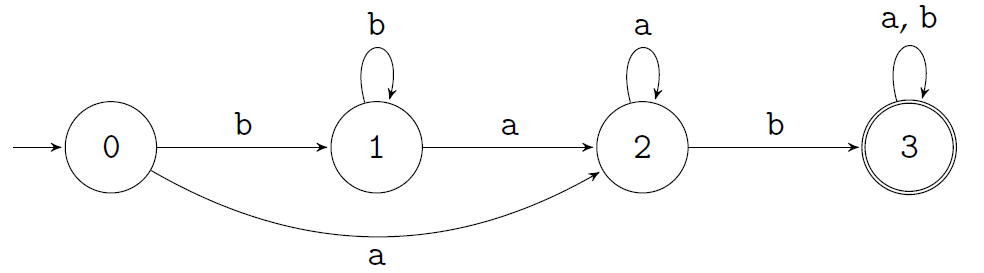
\includegraphics[scale=0.4]{automaten/akz1516B12A1}
	
	Gebt die von $A$ akzeptierte Sprache $L(A)$ unter ausschließlicher Benutzung der formalen Sprachen $\{\word a\}$, $\{\word b\}$, sowie $\{\word a, \word b\}$, des Konkatenationsabschlusses und des Produkts formaler Sprachen an.
	
	\emph{Beispiel:} $\{\word a, \word b\}^* \cdot \{\word a\} \cdot \{\word b\}$
	
	\visible<2-|handout:2>{
		\begin{block}{Lösung}
			$L(A) = \{\word b\}^* \cdot \{\word a\} \cdot \{\word a\}^* \cdot \{\word b\} \cdot \{\word a, \word b\}^*$ \\
			$\hphantom{L(A) } = \{\word b\}^* \cdot \hphantom{\{\word a\} \cdot \mbox{}} \{\word a\}^+ \!\cdot \{\word b\} \cdot \{\word a, \word b\}^*$
		\end{block}
	}
\end{frame}

\begin{frame}{Aufgabe}
	\begin{enumerate}[a)]
		\item Zeichnet einen möglichst kleinen endlichen Akzeptor mit $ X = \{\word a, \word b\}$, der alle Wörter akzeptiert, bei denen die Anzahl der $\word a$ durch $5$ teilbar ist.
		\item Zeichnet einen Akzeptor mit $ X = \{\word a,\word b\}$, der alle Wörter akzeptiert, in denen nirgends hintereinander zwei $\word b$ vorkommen.
	\end{enumerate}		
\end{frame}

\begin{frame} {Lösung a)}
	\begin{figure}[H] 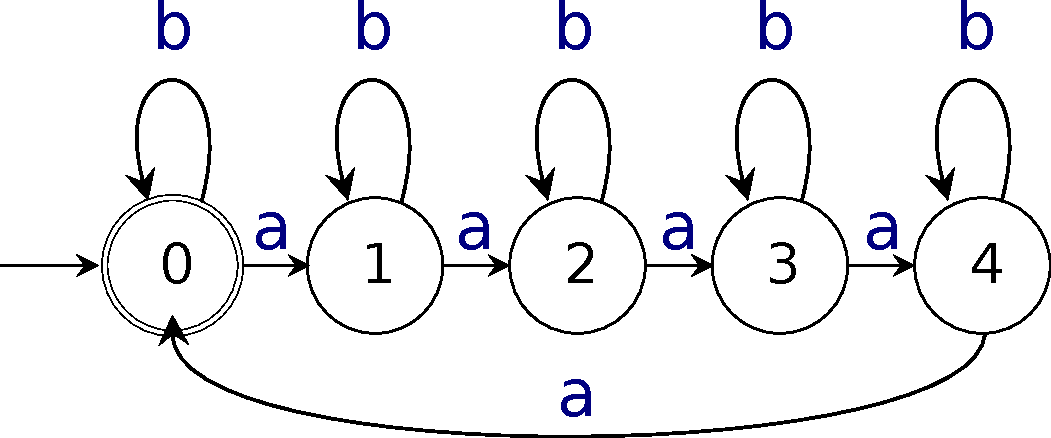
\includegraphics[scale=0.5]{automaten/Akzeptor1.pdf} \end{figure}		
\end{frame} 

\begin{frame}{Lösung b)}
	\begin{figure}[H] 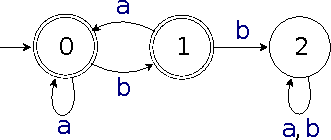
\includegraphics[scale=1.5]{automaten/Akzeptor2.pdf} \end{figure}
\end{frame}

